\subsection{Vertex reconstruction}
In $pp$ collisions, where the charged-particle multiplicity is low, the vertex finding algorithm sometimes fails to find a primary vertex. In addition, at high luminosity, vertex finder can fail due to the contribution of pile-up events and providing a wrong reconstructed vertex. In this study we require at least two reconstructed global tracks $N^{global}_{reco}\geq 2$ passing all the quality cuts listed in Table \ref{tab:trackCut} but without $\textrm{DCA}_{xy}$ and $\textrm{DCA}_{z}$ cuts. 

\subsubsection{Track quality cuts used for vertexing}
A global track  used in vertex reconstruction has to pass the quality cuts listed in the Table \ref{tab:trackCutVertex}, which are different than used in the analysis. Since that, vertex reconstruction efficiency and fake vertex rate is calculated as a function of number of global tracks used in vertexing $N^{global}_{vrt}$ instead of $N^{global}_{reco}$. 


\begin{table}[H]
	\centering
	\begin{tabular}{| l | l |}
		\hline			
		Quantity & Cut \\
		\hline
		\hline
		Number of Fit Points & Fit Points $>20$\\
		Transverse Impact Parameter & $|d_0|<2$~cm\\ 
		Ratio of Fit Points / Possible Fit Points & Fit Points/ Possible Fit Points $>0.52$\\
		Global Track Transverse Momentum & $p_{T}>0.2$~GeV/c\\
		TOF Matched Track & TOF Match-Flag $\geq1$\\
		\hline  
	\end{tabular}
	\caption[Vertexing Track Level Cuts]{Vertexing Track Level Cuts}
	\label{tab:trackCutVertex}
\end{table}
\subsubsection{Vertex efficiency and fake vertex}
In every MC event there is a well defined primary vertex. With the embedded
event reconstructed and the MC information in hand,
the vertex-finding efficiency can be obtained. In the analysis we require exactly one reconstructed vertex with at least two primary tracks passing the selection cuts $N_{reco}^{primary}\geq 2$. The overall
vertex-finding efficiency, $\epsilon_{vrt}^ {best}\left(N_{vrt}^{global}\right)$, is determined as the
ratio of the number of good reconstructed events (reconstructed exactly one primary vertex with at least two primary TOF-matched tracks passing the quality cuts $N_{reco}^{primary}\geq 2$) to the number of input MC events. The fake vertex
rate, $\delta_{vrt}^{fake}\left(N_{vrt}^{global}\right)$, is obtained by the ratio of the number
of fake vertex events to the number of input MC events
\begin{figure}[hb]
	\centering
	\parbox{0.484\textwidth}{
		\centering
		\begin{subfigure}[b]{\linewidth}{
				\subcaptionbox{\label{fig:vertexingEffi}}{\includegraphics[width=\linewidth, page=2]{graphics/vertexing/vertexEffi.pdf}}}
		\end{subfigure}
	}
	\quad
	\parbox{0.484\textwidth}{
		\centering
		\begin{subfigure}[b]{\linewidth}{
				\subcaptionbox{\label{fig:vertexingFake}}{\includegraphics[width=\linewidth, page=3]{graphics/vertexing/vertexEffi.pdf}}}
		\end{subfigure}
	}\\
	\parbox{0.484\textwidth}{
		\centering
		\begin{subfigure}[b]{\linewidth}{
				\subcaptionbox{\label{fig:vertexingEffiZ}}{\includegraphics[width=\linewidth, page=20]{graphics/vertexing/vertexEffi.pdf}}}
		\end{subfigure}
	}
	\quad
	\parbox{0.484\textwidth}{
		\centering
		\begin{subfigure}[b]{\linewidth}{
				\subcaptionbox{\label{fig:vertexingFakeZ}}{\includegraphics[width=\linewidth, page=21]{graphics/vertexing/vertexEffi.pdf}}}
		\end{subfigure}
	}
	\caption[Diagrams of Central Diffraction and Single Diffraction]{Diagrams of Central Diffraction (a) and Single Diffraction (b).}
	\label{fig:vertexEfficiency}
\end{figure}